% ----- PREAMBLE -----

\documentclass[12pt,journal,compsoc]{IEEEtran}

% Package for code syntax
\usepackage{listings}
\usepackage{amsmath} % For code text wrapping
\usepackage{xcolor} % For code text wrapping
\lstset{language=MatLab}

% Package for drawing pictures
\usepackage{graphicx}
\graphicspath{{./Assets/}} % Path to pictures

\providecommand{\PSforPDF}[1]{#1}

\newcommand\MYhyperrefoptions{bookmarks=true,bookmarksnumbered=true,
pdfpagemode={UseOutlines},plainpages=false,pdfpagelabels=true,
colorlinks=true,linkcolor={black},citecolor={black},pagecolor={black},
urlcolor={black},
pdftitle={Machine Learning Techniques for Sentiment Analysis},
pdfsubject={Sentiment Aanalysis, Machine Learning},
pdfauthor={Krystof Hruby},
pdfkeywords={Sentiment Analysis, Machine Learning, Support Vector Machine}}


% ----- DOCUMENT -----

\begin{document}

\title{Machine Learning Techniques\\for Sentiment Analysis}

\author{Krystof Hruby (W20021203)}

\markboth{KF5042 Intelligent Systems, Northumbria University Newcastle}{}


% --- Abstract --- 
\IEEEcompsoctitleabstractindextext{
  \begin{abstract}
    Sentiment analysis is a subfield of the field of natural language processing, whose aim is to obtain sentiment from statements. It has a plethora of applications, particularly in market research, and as such is thus extensively researched and studied by many professionals. Many different machine learning algorithms have been proposed and utilized for sentiment analysis in the past years.

    This paper explores the field of sentiment analysis, its uses in various domains, the complications and problems it faces, and contrasting approaches and algorithms used to solve them. It also showcases the use of an elementary sentiment classifier, using support vector machine as its training and classification algorithm, and analyses its performance and the performance of similar algorithms used in the field.
  \end{abstract}

  \begin{IEEEkeywords}
    Sentiment Analysis, Machine Learning, Support Vector Machine
  \end{IEEEkeywords}}


% --- Maketitle ---
\maketitle

\IEEEdisplaynotcompsoctitleabstractindextext

\IEEEpeerreviewmaketitle


% --- Introduction ---
\section{Introduction}

\IEEEPARstart{S}{entiment} analysis is a technique which allows computers to obtain sentiment (attitudes, feelings, emotions) from human-created text. It is occasionally referred to as “opinion mining”, but some sources differentiate between the two terms [11].
Sentiment analysis is a part of natural language processing field. Natural language processing aims to allow computers to understand – obtain meaning from human text/speech, or produce content related to human language and written word.

Very often a purely objective examination of human language by a machine is not enough to dissect the true context behind it. Similar sentences can have different, even opposite, meanings depending on the way they are phrased (e.g., sarcasm). On top of that, sometimes, the emotions expressed (e.g., disappointment, satisfaction) are more valuable than the content itself and thus, sentiment analysis is not just a helpful tool for the synthesis of human-language in general but has many applications in various fields.

E-commerce and online shopping have become an undisputable part of modern global market – according to Statista [2], retail internet sales have accounted for almost five trillion USD (almost 4 trillion GBP) and are projected to gain the share of 25\% of total global retail sales by 2025. The weight of online markets has been even more amplified by the Covid-19 pandemic. Users often decide between products based on their reviews or comments/posts on social media or online articles [5], [15]. Through sentiment analysis techniques, this data can be examined and used for market research [4], [5], [15]. Understanding of opinions about products and their features can greatly assist retailers in business decisions.

Opinions voiced on social media sites can be used with sentiment analysis in other cases too. Since the internet has become a major platform for political candidates, parties or movements, whose supporters or opponents are willing to openly share their thoughts through social media, sentiment analysis can help to identify potential voters or platforms or serve as an analysis tool for polls and predictions [4] [5].
While used seldomly in such cases at this time, sentiment analysis can also prove applicable in mental health diagnosis or mental health studying. Wang et al [20] have developed a sentiment analysis model that attempts to detect signs of depression of social media users in China.

Due to its breadth of applications and their significance, sentiment analysis is one of the most prominent research areas in machine learning and computer science. Feldman [5] counts over 700 articles that have been written on the topic and that “hundreds of start-ups are developing sentiment analysis solutions”.
Sentiment analysis is regarded as a classification problem. Three major classification levels are usually categorized in sentiment analysis: document-level, sentence-level, and aspect-level. Many different sentiment analysis algorithms and enhancements were proposed in the last couple of years [11]. These are divided into machine-learning or lexicon-based methods or their combinations. Different approaches and their applications are further described below in section “Literature Review”.

% --- Literature Review ---
\section{Literature Review}
There are many different techniques (and their combinations) used for different problems in sentiment analysis. Medhat et al [11] and Prabowo and Thelwall [16] have collected a survey of many diverse models, their training data sets and use cases; Zhang et al [22] have described several deep learning algorithms applicable for sentiment analysis; some more sentiment analysis tools and techniques can be also found in [1] and [4].

Due to its nature, sentiment analysis algorithms differ in various ways. Even the classification itself can be either binary – negative and positive (and neutral in some cases), or a scale - from negative value to positive value (in percentage for example). Moreover, this scale can be divided into different number of points, for example a model by Pang and Lee, noted in [16, Table 2] assigns sentiments using a 3- or 4-point scale.

\subsection{Document, Sentence and Aspect Level}
As mentioned above, sentiment analysis is divided into three main classification levels. Document-level sentiment analysis aims to classify (assign negative/positive sentiment to) a whole document. Sentence-level sentiment analysis focuses only on the sentiment of a sentence or a small portion of text. Aspect-level sentiment analysis tries to also differentiate between different aspects and the sentiments expressed regarding them. An example sentence for aspect-level sentiment analysis from [11]: “The voice quality of this phone is not good, but the battery life is long”.

Since document- and sentence-level sentiment analysis do not differentiate between aspects included in them, they may often not provide the necessary details [5], [11]. This is the main reason for why aspect-level sentiment analysis may be used over document- and sentence-level sentiment analysis despite being generally more difficult.

In some cases, traditional sentiment analysis using one the three aforementioned methods cannot be used, and a comparative sentiment analysis must be applied instead. Comparative sentiment analysis aims to classify sentiments from comparative statements (i.e., X is better than Y) and the preferred items. An example sentence for comparative sentiment analysis from [5]: “300 C Touring looks so much better than the Magnum”.

\subsection{Machine Learning and Lexicon-Based Approach}
Approaches to sentiment analysis include machine learning and lexicon-based algorithms. Machine learning approaches utilize machine learning models built for sentiment analysis. Lexicon-based approaches are dependent on a sentiment lexicon – a collection of pre-processed text with known sentiment classification.

Machine learning approaches tend to be more accurate, however they require a training phase, which must be conducted before they can be utilized [4]. Lexicon-base approaches, on the other hand, do not have any such limitations and are thus more widely utilized by the marketing research community [4]. Machine learning approaches can be then further divided into supervised and unsupervised learning, lexicon-based approaches into dictionary- and corpus-based [11]. Hybrids and combinations of both approaches can be also used in some cases [4], [11], [16].

Below are some examples of algorithms utilized in the domain of sentiment analysis and their brief descriptions.

\subsection{Naïve Bayes and Bayesian Network}
Naïve Bayes is a famous machine learning algorithm, which calculates weights for each feature of a class and then, based on that, deduces probability for each corresponding class – the item with the highest calculated probability is then selected as the prediction. It is a probabilistic classifier and [11] describes it as the simplest and most commonly used sentiment analysis classifier.

Naïve Bayes assumes the independence of classified features, whereas Bayesian network assumes the opposite – all features are completely dependent. The computational complexity of a Bayesian network for sentiment analysis is very expensive and is thus not frequently utilized [11].

Descriptions of Naïve Bayes and Bayesian network can be found in [14] and [6] respectively.

\subsection{Support Vector Machine}
Support vector machine is a linear classifier, and its objective is to classify data by splitting point sets with hyperplanes in an n-dimensional space. Support vector machine is another prominent machine learning algorithm and as such has many uses even outside sentiment analysis. Support vector machines are particularly fitted to be used on text data and have been thus extensively utilized in sentiment analysis [1], [11].

The further parts of this paper describe an elementary sentiment classifier which uses support vector machine as its training algorithm.

\subsection{Nerual Network}
Neural Networks are (to some extent) based on the operations of neurons in the human brain. Each neuron has a different weight and carries some information to other neurons, organized in layers. The training process of a Neural Network utilizes a back-propagation algorithm to adjust weights for the neurons.

According to Zhang et al [22], the advances in hardware and its availability in the past years have made neural networks considerably applied in sentiment analysis and natural language processing.

Descriptions of some specific neural network algorithms utilized in sentiment analysis can be found in [1], [11] and [22].

\subsection{Dictionary-Based and Corpus-Based}
Dictionary-based approaches utilize a manually created word dictionary with positive/negative orientations. This set can be then expanded by searching for synonyms and antonyms [11]. Corpus-based approaches also use a word dictionary, however there is a set of rules and patterns built on top of it, by which the words are classified.

% --- AI Experiments ---
\section{AI Experiments}
The experiments which were conducted showcase an elementary binary sentiment classifier, which uses support vector machine algorithm as its model. The classifier was programmed and developed in MatLab [10]. Datasets used for training the model (and for which were thus the results calculated) were [9], [12] and [13], however the classifier was coded to be universal and can be trained with any (binary) sentiment lexicon. The datasets used contain elementary English words and phrases; some other datasets which can be used are [8] – datasets gathered from top communities on a popular website “reddit” [17] and historical datasets corresponding to past years, and [18] – sentiment datasets for 81 languages.

The sentiment classifier is a class with three public methods – Train, Test and Classify (Appendix A). The Train method takes in the training data and trains a model using the support vector machine algorithm. The Test method takes in the testing data, predicts sentiment of the data with the trained model and compares its prediction with true values, then produces the results as a confusion matrix (true/false positives/negatives) and calculates its accuracy (\begin{math}(true\ positives + true\ negatives) \div (true\ positives + true\ negatives + false\ positives + false\ negatives)\end{math}), precision (\begin{math}true\ positives \div (true\ positives + false\ positives)\end{math}) and recall (\begin{math}true\ positives \div (true\ positives + false\ negatives)\end{math}). The Classify method takes in a text to be classified and predicts its sentiment with the trained model. Demonstration of the sentiment classifier can be seen by running the main function (Appendix B).

\subsection{Support Vector Machine}
The sentiment classifier uses the support vector machine algorithm for its training and subsequent classifying.
Support vector machine is a supervised machine learning algorithm, which creates a non-probabilistic binary (two-class) linear classifier. The objective of a support vector machine is to find an (N-1)-dimensional hyperplane in an N-dimensional space, which separates data points into distinct categories (Appendix C). New data is then classified using this support vector classifier. Support vector machines were first devised by Vladimir Vapnik and his colleagues at AT \& T Bell Laboratories in 1995 [3].

The first step of the algorithm is to represent text as vectors. These are plotted as data points onto a space. The algorithm then calculates a hyperplane with the largest margin between the categories of the data vectors. The points that are the closest to the hyperplane are called support vectors; these points ultimately decide the final orientation of the hyperplane. If the space is 1-dimensional (line), the hyperplane will be a point, if the space is 2-dimensional (plane), the hyperplane will be a line, if the space is 3-dimensional (space), the hyperplane will be a plane, etc.

Due to the nature of data, it may not be possible to create a hyperplane with clear distinction between the categories. To solve this problem, support vector machines make use of so called kernel functions, which systematically find support vector classifiers in higher dimensions. There are many different kinds of kernel functions, such as nonlinear, linear, polynomial, radial (radial basis function) and sigmoid.
The full description of support vector machines can be found in [3]. Visual explanation of support vector machines can be found in [14]. More information about how support vector machines are used within the domain of sentiment analysis and natural language processing can be found in [7], [11] and [21].

% --- Result Analysis ---
\section{Result Analysis}
As mentioned before, support vector machines are believed to be one of the best approaches to sentiment analysis (and natural language processing) and have been thus widely adapted for various tasks in this domain. Medhat et al [11] notes 12 support vector machines (out of 54 sentiment analysis algorithms collected) and Prabowo and Thelwall [16] note 5 (out of 14 sentiment analysis algorithms collected) used in real life scenarios, ranging from movie reviews through tweets (posts on a social media application twitter [19]) to “relationship biography”. Ahmad et al [1] places support vector machines as one of the most accurate sentiment analysis algorithms at around 80\% classification accuracy.

The model tested in this paper achieved 82\% mean accuracy (the amount of true classifications from the total of all elements) with 79\% mean precision (positive predictive value) and 77\% mean (sensitivity) with [9], [12] and [13] as datasets (for both training and testing). The data was gathered over 100 test runs. Since the data in those datasets is compiled only from (English) words and short phrases, it is not strongly representative of real-world uses, where whole sentences and paragraphs (and even articles, books) must be classified.

The classifier reaches high accuracy when applied to words and short phrases, however its accuracy falls at 50\% (at the level of a coinflip), when tried onto sentences or larger text blocks. To mitigate this, the text classified can be pre-processed by tokenizing (splitting sentences into individual words), each word classified separately, and the final result then computed from classifications of the separate words. This approach has a major downside, however, since it does not take negators into account – for example “not good” will be classified as positive (as if it meant “good”, instead of “bad”), which severely diminishes the gains acquired through these means. The model is also unable to dissect aspects, which means it cannot properly classify comparative statements (i.e., “Product X is good, but product Y is not”). A more robust corpus-based algorithm would have to be built upon this model to make it practical in such scenarios. Similar results were recorded by Selamat and Zainuddin [21] with 70\% to 80\% accuracy for unigrams and only 50\%-55\% accuracy for trigrams.

The particular datasets used for training the model also affect performance. When trained with datasets compiled from the most popular communities on reddit [8], the accuracy varied from 70\% to 80\% depending on the specific community datasets. The accuracy of the model trained with language specific datasets [18] ranged even more widely. With some languages, the model was completely unable to correctly categorize positive sentiments (for example Czech, Hungarian), with others, it outperformed the English classifier by significant margins (for example Simplified Chinese). This variance is to be expected, as the datasets are quite modest, and the support vector machine algorithm is thus incapable of building an adequate separation hyperplane. Exact accuracies, precisions and recalls of models trained on these datasets can be found in Appendix D and Appendix E.

% --- Conclusion and Future Work ---
\section{Conclusion and future work}
Sentiment analysis is a major subfield of the field of natural language processing and of the most popular research areas in machine learning and computer science. It has many real world applications and, particularly with the current golden age of social media and online shopping, is likely to become even more prominent in the future.

There are many approaches to creating models for sentiment analysis, ranging from classic ones, such as Naïve Bayes or support vector machines, to more “trendy” ones, such as neural networks. Each have their strengths and weaknesses and must be thus built for specific tasks and with specific training datasets in mind.

Support vector machines are one of the best and most widely adopted algorithms for sentiment analysis, with high classification accuracies for words or short phrases, but with lesser regard for larger texts or aspect-level classification. Using their advantages in a hybrid configuration alongside other algorithms might yield the best results. One of such approaches is described in [22].

% --- Appendix

\newpage  % Put appendix onto a separate page

\appendices
\section{Sentiment Classifier Class}
\begin{lstlisting}[basicstyle=\small, breaklines=true, postbreak=\mbox{\textcolor{red}{$\hookrightarrow$}\space}]
% Sentiment classifier class
% Classifies sentiment of text into Positive, Negative and Neutral
% Uses support vector machine for its model
classdef SentimentClassifier < handle
    % PRIVATE PROPERTIES
    properties (Access = private)
        FTWEmbedding
        Model
    end

    % PUBLIC PROPERTIES
    properties (Access = public)
        ClassificationAccuracy
        ClassificationPrecision
        ClassificationRecall
    end

    % PUBLIC METHODS
    methods (Access = public)
        % Constructor
        function obj = SentimentClassifier()
            % Load fastTextWordEmbedding toolbox
            % https://www.mathworks.com/help/textanalytics/ref/fasttextwordembedding.html
            obj.FTWEmbedding = fastTextWordEmbedding;
        end

        % Trains the model on parameter data
        function obj = Train(obj, data)
            % Remove words that are not included in FTWEmbedding
            removedWords = ~isVocabularyWord(obj.FTWEmbedding, data.Text);
            data(removedWords,:) = [];

            % Convert text into word-vectors using word2vec from fastTextWordEmbedding toolbox
            data_WordVectors = word2vec(obj.FTWEmbedding, data.Text);

            % Train the model for binary classification using fitcsvm
            % https://www.mathworks.com/help/stats/fitcsvm.html
            obj.Model = fitcsvm(data_WordVectors, data.Label);
        end

        % Tests the classifier on known data and shows the results as a confusion matrix and its accuracy
        function [obj, prediction] = Test(obj, data, visualize)
            % Convert words into word-vectors using word2vec from fastTextWordEmbedding toolbox
            predictionData_WordVectors = word2vec(obj.FTWEmbedding, data.Text);
            
            % Predict the sentiment
            [prediction, ~] = predict(obj.Model, predictionData_WordVectors);

            % Create confusion matrix for the classification
            confusionMatrix = confusionmat(data.Label, prediction);
            truePositives = confusionMatrix(1,1);
            trueNegatives = confusionMatrix(2,2);
            falsePositives = confusionMatrix(1,2);
            falseNegatives = confusionMatrix(2,1);
            classificationAccuracy = (truePositives + trueNegatives) / (truePositives + trueNegatives + falsePositives + falseNegatives) * 100;
            classificationPrecision = truePositives / (truePositives + falsePositives) * 100;
            classificationRecall = truePositives / (truePositives + falseNegatives) * 100;

            obj.ClassificationAccuracy = classificationAccuracy;
            obj.ClassificationPrecision = classificationPrecision;
            obj.ClassificationRecall= classificationRecall;

            % Print the confusion matrix and accuracy onto the console
            fprintf("True positives: %d\n", truePositives);
            fprintf("True negatives: %d\n", trueNegatives);
            fprintf("False positives: %d\n", falsePositives);
            fprintf("False negatives: %d\n", falseNegatives);
            fprintf("Accuracy: %d\n", round(classificationAccuracy));
            fprintf("Precision: %d\n", round(classificationPrecision));
            fprintf("Recall: %d\n", round(classificationRecall));

            % Visualize the confusion matrix
            if nargin == 3 && visualize == "visualize"
                figure
                confusionchart(data.Label, prediction);
            end
        end

        % Classifies sentiment of data
        function prediction = Classify(obj, text)
            % Convert text into word-vectors using word2vec from fastTextWordEmbedding toolbox
            data_WordVectors = word2vec(obj.FTWEmbedding, text);

            % Predict the sentiment
            [prediction,~] = predict(obj.Model, data_WordVectors);

            % Print the prediction onto the console
            fprintf("%s => %s\n", text, prediction);
        end
    end
end
\end{lstlisting}

\section{Main Function}
\begin{lstlisting}[basicstyle=\small, breaklines=true, postbreak=\mbox{\textcolor{red}{$\hookrightarrow$}\space}]
% Clear workspace and console
clc; clear;

% Load training data from a lexicon into the workspace
data = loadLexicon;

% Split data into training and testing sets
testingAmount = 0.05; % 5% reserved for testing
[data_Training, data_Testing] = splitData(data, testingAmount);

% Create a sentiment classifier (class)
sentimentClassifier = SentimentClassifier;

% Train the sentiment classifier
sentimentClassifier.Train(data_Training);

% Test the sentiment classifier
% Calculates the confusion matrix and accuracy of the trained model
sentimentClassifier.Test(data_Testing, "visualize");

% Example use of the classifier (can be used once trained):
textData = "The product was not very good.";
sentimentClassifier.Classify(textData);
\end{lstlisting}

\newpage % Put other appendices on a separate page

\section{Support Vector Machine}
This graph showcases the classification technique of a support vector machine. A hyperplane with the largest margin from both sets of data points separates data into two distinct categories.

The blue and red circles represent individual data points (with 2 classified features). The green line represents the classification hyperplane (in a 2-dimensional space a line).
\begin{center}
  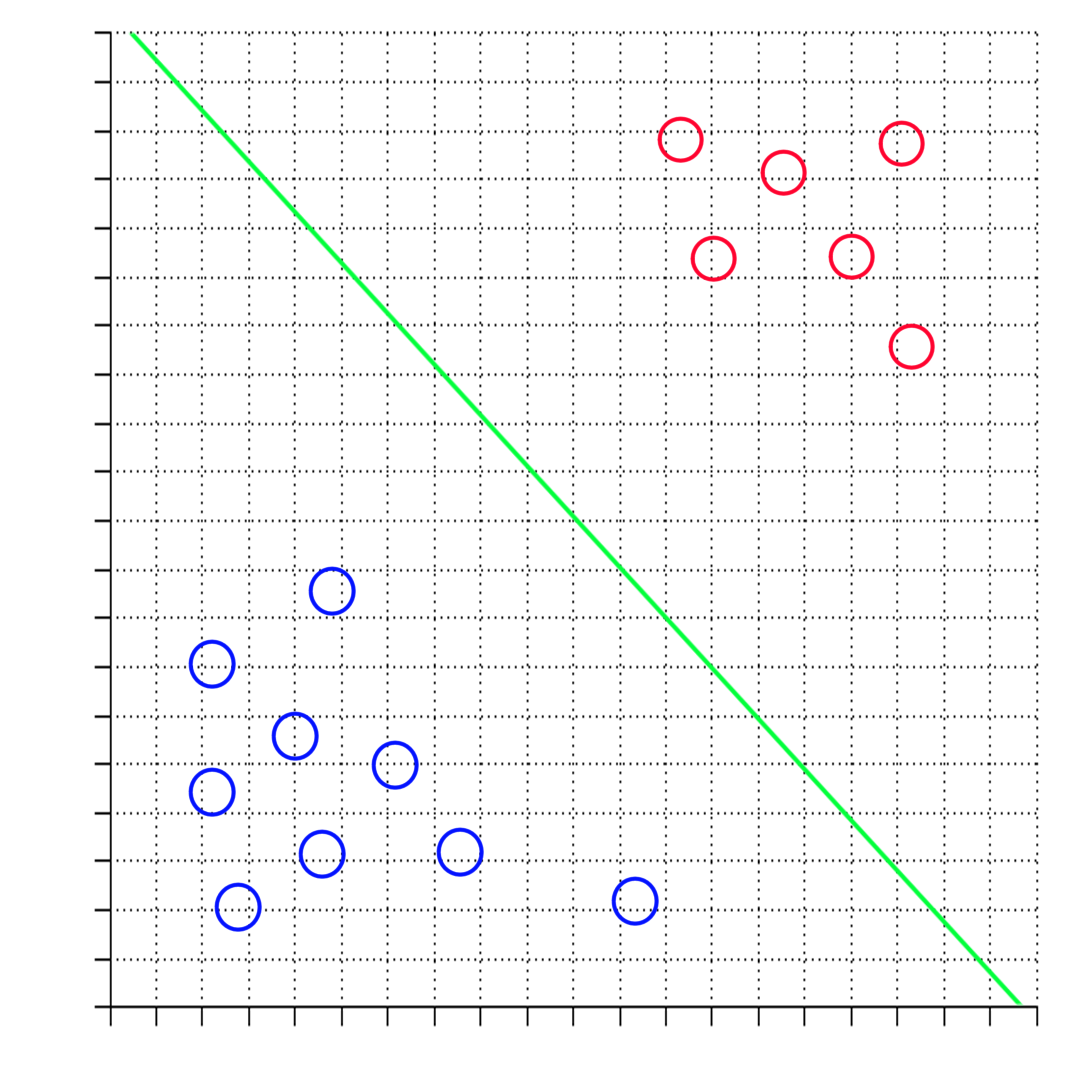
\includegraphics[scale=1.7]{support-vector-machine-showcase-graph.png}
\end{center}

\section{Reddit Communities Datasets}
\begin{center}
  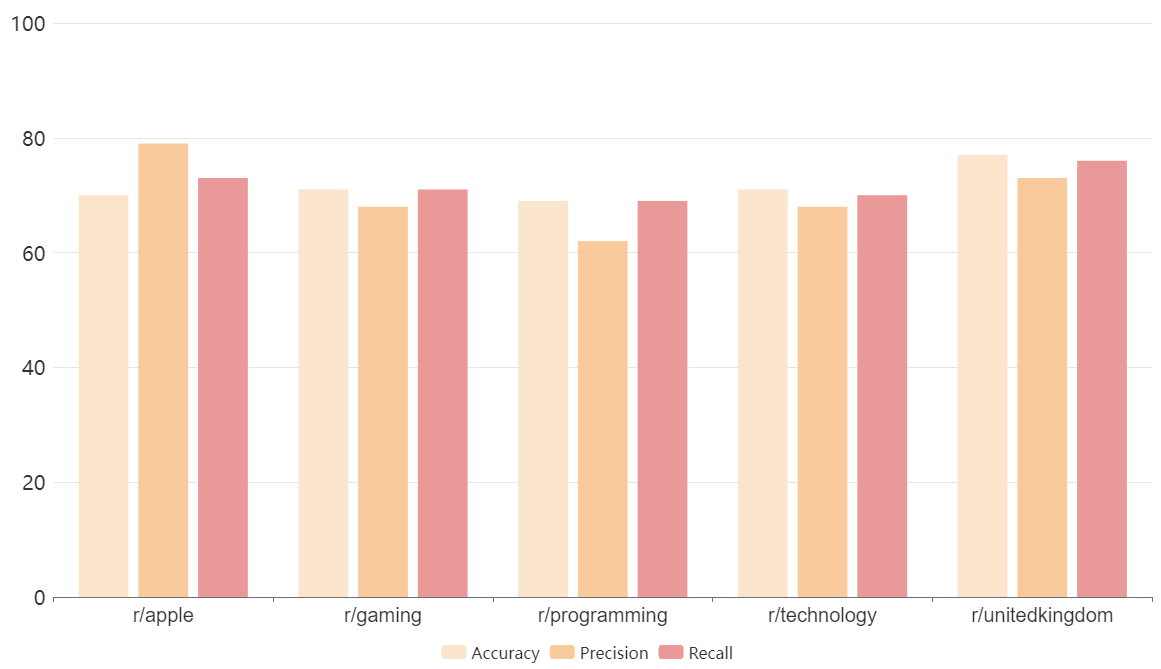
\includegraphics[scale=0.24]{reddit-communities-datasets.png}
\end{center}

\newpage % Fix page spacing

\section{World Languages Datasets}
\begin{center}
  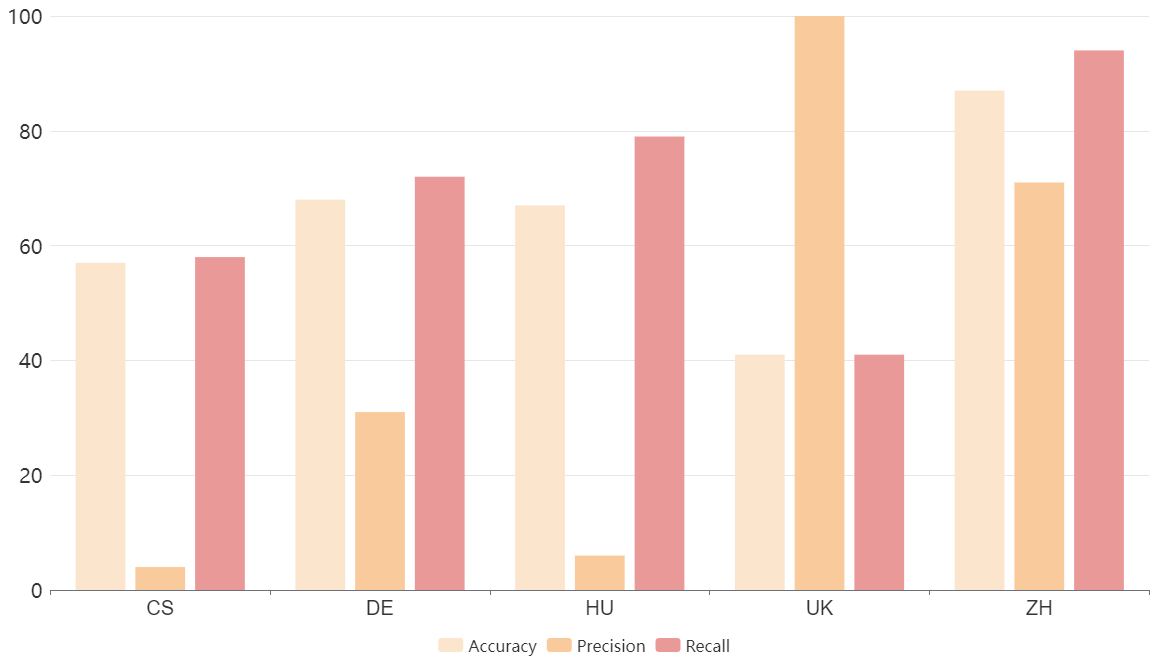
\includegraphics[scale=0.24]{world-languages-datasets.png}
\end{center}

% --- References ---

\newpage % Put references onto a separate page

\begin{thebibliography}{1}
  \bibitem{}
  Ahmad M. \emph{et al.}, “Machine Learning Techniques for Sentiment Analysis: A review,” International Journal of Multidisciplinary Sciences and Engineering, vol. 8, no. 3, pp. 27-32, Apr. 2017.

  \bibitem{}
  Coppola D., \emph{E-commerce worldwide – statistics \& facts}, Statista, Feb. 2022. Accessed on May. 5, 2022. [Online]. Available: https://://www.statista.com/topics/871/online-shopping/\#topicHeader\_\_wrapper.

  \bibitem{}
  Corinna, C. and Vapnik V., “Support vector Networks,” \emph{Mach Learn 20}, pp. 273-297, Sep. 1995, doi: 10.1007/BF00994018.

  \bibitem{}
  Dhaoui Ch. \emph{et al.}, “Social media sentiment analysis: lexicon versus machine learning,” \emph{Journal of Consumer Marketing}, vol. 34, no. 6, pp. 480-488, Sep. 2017.

  \bibitem{}
  Feldman R., “Techniques and Applications for Sentiment Analysis,” \emph{Communications of the ACM}, vol. 56, no. 4, pp. 82-89, Apr. 2013.

  \bibitem{}
  Friedman N. \emph{et al.}, “Bayesian Network Classifiers,” \emph{Machine Learning 29}, pp. 131-163, Nov. 1997, doi: 10.1023/A:1007465528199.

  \bibitem{}
  Gaurangi P. \emph{et al.}, “Sentiment Analysis Using Support Vector Machine,” \emph{International Journal of Innovative Research in Computer and Communication Engineering}, vol. 2, no. 1, pp. 2607-2612, Jan. 2014.

  \bibitem{}
  Hamilton W. L. \emph{et al.}, “SocialSent: Domain-Specific Sentiment Lexicons for Computational Social Science.” 2016. https://nlp.stanford.edu/projects/socialsent/

  \bibitem{}
  Hu M. and Bing L., “A list of English positive and negative opinion words or sentiment words.” 2004. http://www.cs.uic.edu/~liub/FBS/opinion-lexicon-English.rar

  \bibitem{}
  \emph{MatLab}. (R2021b). MathWorks. Available: https://uk.mathworks.com/products/matlab.html

  \bibitem{}
  Medhat W. \emph{et al.}, “Sentiment analysis algorithms and applications: A survey,” Ain Shams Engineering Journal, vol. 5, no. 4, pp. 1093-1113, Dec. 2014.

  \bibitem{}
  Mohammad S. M. and Kiritchenko S., “Sentiment Composition Lexicon of Negators, Modals, and Adverbs (SCL-NMA).” 2016. http://saifmohammad.com/WebDocs/lexiconstoreleaseo \newline nsclpage/SCL-NMA.zip

  \bibitem{}
  Mohammad S. M. and Kiritchenko S., “Sentiment Composition Lexicon of Opposing Polarity Phrases (SCL-OPP).” 2016. http://saifmohammad.com/WebDocs/lexiconstoreleaseo \newline nsclpage/SCL-OPP.zip

  \bibitem{}
  Murphy K. P., “Naïve Bayes classifiers,” University of British Columbia, Oct. 2006

  \bibitem{}
  Popescu Ana-M. and Etzioni O., “Extracting Product Features and Opinions from Reviews,” in Natural Language Processing and Text Mining. London, The United Kingdom of Great Britain and Northern Ireland: Springer, 2007, ch. 2, pp. 9-28.

  \bibitem{}
  Prabowo R. and Thelwall M., “Sentiment analysis: A combined approach,” \emph{Journal of Informetrics}, vol. 3, no. 3, pp. 143-157, Apr. 2009.

  \bibitem{}
  \emph{Reddit}. Reddit Inc. [Online] Available: https://www.reddit.com

  \bibitem{}
  Tatman R., “Sentiment Lexicons for 81 languages.” 2017. https://sites.google.com/site/datascienceslab/projects/m \newline ultilingualsentiment

  \bibitem{}
  \emph{Twitter}. Twitter, Inc. [Online] Available: https://twitter.com

  \bibitem{}
  Wang X. \emph{et al.}, “A Depression Detection Model Based on Sentiment Analysis in Micro-blog Social Network,” presented at Pacific-Asia Conference on Knowledge Discovery and Data Mining, Heidelberg, Berlin: Springer, pp. 201-213, 2013.

  \bibitem{}
  Zainuddin N. and Selamat A., “Sentiment analysis using Support Vector Machine,” in 2014 International Conference on Computer Communication, and Control Technology (I4CT). Langkawi, Malaysia: Institute of Electrical and Electronics Engineers Malaysia Section, 2014, pp. 333-337. Doi: 10.1109/I4CT.2014.6914200.

  \bibitem{}
  Zhang L. et al, “Deep learning for sentiment analysis: A survey,” \emph{WIREs Data Mining and Knowledge Discovery}, vol. 8, no. 4, Mar. 2018.
\end{thebibliography}

\end{document}